\part{A Crush Course on CFT}
% 计数器清零,每个part都要引用,除了part1
\setcounter{theorem}{0}
\setcounter{definition}{0}
\setcounter{lemma}{0}
\setcounter{sidenote}{1}

CFT经典教材是大黄书\cite{DiFrancesco:1997nk},教材\cite{Blumenhagen:2009zz,ito}也是不错的选择\sn{伊藤克司先生的书还没有官方中文译本,不过这里有民间译本的重排本\url{https://github.com/WHUZBF/CFT-book}},还有一些比较好的讲义\cite{Nawata:2022lsw,Ginsparg:1988ui,Qualls:2015qjb},共形场论的自举(bootstrap)方法也是非常重要的,可以见讲义\cite{Ribault:2014hia}的专门介绍。CFT也可以当作一门数学课来学习,偏重于数学的阅读材料有\cite{Schottenloher:2008zz}。

首先是一些Overview性质的介绍。CFT无非就是一种特殊的QFT,但是这个时候理论具有比Poincar\'e对称性更大的对称性,在二维的情况下甚至提升为无穷维的对称性,这种对称性能让我们不通过微扰场论直接确定关联函数。一般的QFT中我们用Poincar\'e的不同的不可约表示来标记不同的场,或者说,我们用自旋来标记场,到了CFT这边,我们还需要使用共形维数$\Delta$来标记,对于$s=0$的标量场,共形维数定义为在Dilation $x\mapsto\lambda x$ 下场变换为:
\begin{equation}
	\phi^\prime(\lambda \vec{x})=\lambda^{-\Delta}\phi(\vec x)
\end{equation}
但是这只是对Dilation要求场在共形变换下“协变”,进一步要求对任意共形变换“协变”就给出了\textbf{初级场}(primary field)的定义。\sn{注意我们遵从大黄书的符号约定,和\cite{Blumenhagen:2009zz,,Ginsparg:1988ui}的定义恰巧相反,对最终CFT中的一些结论没有任何影响,仅仅只是中间推导过程有些细微的差别。}\sn{$s=1/2$是何形式?}
\begin{definition}
	共形维数为$\Delta$的初级场(s=0)定义为在任意共形变换下满足:
	\begin{equation}
		\phi^\prime(\vec{x^\prime})=\left|\frac{\partial \vec {x^\prime}}{\partial \vec {x}}\right|^{\Delta/d}\phi(\vec {x})
	\end{equation}
\end{definition}

初级场将是后面研究的主要对象。二维的共形对称性比较特殊,分为global和local的,如果上面的“协变性”只对global的共形变换适用,那我们称之为\textbf{准初级场}(quasi-primary field),显然初级场一定是准初级场,反过来却不一定。二维情况下我们还使用复平面为坐标\footnote{这是欧氏空间CFT的主要选取,也是后文研究的主要内容,Wick转动到闵氏时空之后选取所谓光锥坐标。},但是我们为了一些地方的方便,并不是考虑的$\mathbb{C}$,而是$\mathbb{C}^2$,也就是说我们把$z,\bar z$看作是完全独立的变量,进在一些特殊情况下认为$z^*=\bar z$。而且把$\Delta$拆分为共形权$(h,\bar h)=\frac{1}{2}\left(\Delta+s,\Delta-s\right)$在这一符号约定下,共形权定义变为:
\begin{equation}
	\boxed{
	\phi^{\prime}(\lambda z,\overline{\lambda}\overline{z})=\lambda^{-h}\overline{\lambda}^{-\overline{h}}\phi(z,\overline{z})
	}
\end{equation}
(准)初级场定义变为:
\begin{equation}
	\boxed{
		\phi^{\prime}\left(f(z),\overline{f}(\overline{z})\right)=\left(\frac{\partial f}{\partial z}\right)^{-h}\left(\frac{\partial\overline{f}}{\partial\bar{z}}\right)^{\overline{-h}}\phi(z,\bar{z})
	}
\end{equation}
如果$\phi$全纯我们称为\textbf{chiral},反全纯称为\textbf{anti-chiral}。无穷小共形变换$x\mapsto x+\epsilon$下:
\begin{equation}\label{ict}
	\boxed{
	\delta_{\epsilon,\bar{\epsilon}}\phi(z,\bar{z})\equiv\phi^\prime(x^\prime)-\phi(x)=-\left(h\mathrm{~}\partial_z\epsilon+\epsilon\mathrm{~}\partial_z+\overline{h}\mathrm{~}\partial_{\bar{z}}\bar{\epsilon}+\overline{\epsilon}\mathrm{~}\partial_{\bar{z}}\right)\phi(z,\overline{z})
	}
\end{equation}
\begin{remark}
	初级场的定义可以看作是一种拓宽的张量定义,考虑一个带$s$个协变指标的张量,在任意坐标变换$x\mapsto x+\epsilon(x)$下:
	\[-\delta\Phi_{\mu_1\cdots\mu_s}=\epsilon^\nu\partial_\nu\Phi_{\mu_1\cdots\mu_s}+(\partial_{\mu_1}\epsilon^\nu)\Phi_{\nu\mu_2\cdots\mu_s}+\cdots+(\partial_{\mu_s}\epsilon^\nu)\Phi_{\mu_1\cdots\mu_{s-1}\nu}\]
	换到复平面,简单起见只考虑全纯部分,那么$h=s$,上面的定义局限于$h$是整数,现在考虑任意取值,那些指标也没必要写出了,便得到:
	\[-\delta\Phi=\epsilon\partial\Phi+s\partial \epsilon\Phi\]
	这就是前面得到的无穷小变换形式。
\end{remark}

同QFT一样,这些场都会量子化成算符。不像QFT中我们研究的场是有限多个的,比如说QED就是正负电子对应的Dirac场和一个U(1)规范场耦合,CFT中我们研究的场很多情况下会是无穷多个的,因为我们把$\phi,\partial\phi$看作是不同的场,因为他们是不同共形权的初级场。定义一个CFT第一步就是告诉我们理论中有哪些初级场,也就是一个\textbf{谱}(Spectrum)$\{\mathcal{O}_{h,\bar h}\}$。CFT中我们并非按照微扰场论那一套来建立关联函数的计算方法的,而会去关注场之间的\textbf{算符乘积展开(OPE)},后面将会看到自举给出了OPE的绝大多数信息,还有一些系数是自举无法确定的,需要CFT的定义给定,这是定义CFT的第二个data。我们这样做是在算符的观点下看问题,或者说是在海森堡表象下看问题,那CFT的态是什么呢?这其实被所谓\textbf{态算符对应}联系起来。

最后想强调一点,正是因为CFT的思考方式和一般的QFT有比较大的不同,所以CFT的建立甚至是不需要已知理论的拉氏量的,我们需要知道的只是理论拥有的对称性,然后去找对称性的表示构造谱,能动量张量则刻画了CFT在共形变换下的性质,是构建OPE必须的,如果强行利用拉格朗日量进行分析反而会变得非常复杂,有的CFT甚至是没办法写下一个拉氏量的,但是通过自洽性分析我们是知道这种理论的存在性的,而且可以根据自举方法走得很远。

\section{Virasoro Algebra}
讨论共形场论,都是在量子层面上已经消去共形反常后的理论,比如YM理论就是量子化后存在共形反常的QFT,从而不能看作一个CFT。二维CFT的共形代数是$\mathrm{Witt}\times\overline{\mathrm{Witt}}$,后面我们讨论CFT其实都是在其中心扩张$\mathrm{Vir_c}\times\overline{\mathrm{Vir_c}}$下进行\sn{明确一下convention,扩张前的代数用小写$l$标记,扩张后的用大写$L$标记}。这里我不打算讨论过多中心荷的物理意义,这应当是弦论课的内容,为何要引入中心荷可以从群表示的观点来看。

首先如果一个CFT具有某个对称性,这个对称性构成了一个群,那么体系的谱就生活在这个群的群表示之中\sn{严格说是表示的最高权是那些初级场,也就是CFT的谱,由这些谱生成的次级态最终张成整个CFT的希尔伯特空间,也就是对称代数的表示。}。也就是说假设对称代数为$\mathfrak{V}\times\bar{\mathfrak{V}}$\sn{注意在二维CFT中我们都会将对称代数复化为两个独立的部分。两个独立的李代数可以作为线性空间考虑他们的直和$\mathfrak{V}\oplus\bar{\mathfrak{V}}$,这里写成$\times$也没错,是将他们考虑成集合,然后做卡氏积,由于两部分独立,所以这两者本质上没区别。},则:
\begin{equation}
	\boxed{\mathcal{S}=\bigoplus_{(\mathcal{R},\mathcal{R}^{\prime})\in\mathrm{Rep}(\mathfrak{V})^2}m_{\mathcal{R},\mathcal{R}^{\prime}}\mathcal{R}\otimes\bar{\mathcal{R}^{\prime}}}
\end{equation}
但是这个表示只需要是个射影表示就好,而射影表示对应的是李代数的中心扩张的表示。前面处理洛伦兹群我们不用考虑那么多,因为我们这证明了理论总是可以redefine来消去中心荷,但是一般的共形场论至少都有Virasoro对称性,而这个代数的中心荷是non-trivial的,一般是不能消除的,所以我们考虑对称性并非直接考虑$\mathrm{Vir}$,而是$\mathrm{Vir}_c$。
\begin{theorem}[Virasoro Algebra]
	\begin{equation}
		\boxed{
		\left[L_m,L_n\right]=\left(m-n\right)L_{m+n}+\frac c{12}\left(m^3-m\right)\delta_{m+n,0}
		}
	\end{equation}
\end{theorem}
\begin{remark}
	如果我们考虑$\mathfrak{sl}(2,\mathbbm{C})$子代数,会发现中心扩张是trivial的。
\end{remark}
\section{Radial Quantization and Hilbert Space}
\subsection{Radial Quantization}
对于$1+1$维时空,可以把空间方向一点紧化为圆,这样平面就会变为一个圆柱面,这样就可以引入圆柱面上的复坐标$w=x^0+ix^1$,这样$w\sim w+2\pi i$自动满足周期性条件,这也是弦论worldsheet的图像。而圆柱面又可以通过共形变换$w\mapsto e^w$变到另一个复平面上:
\begin{figure}[htbp]
	\centering
	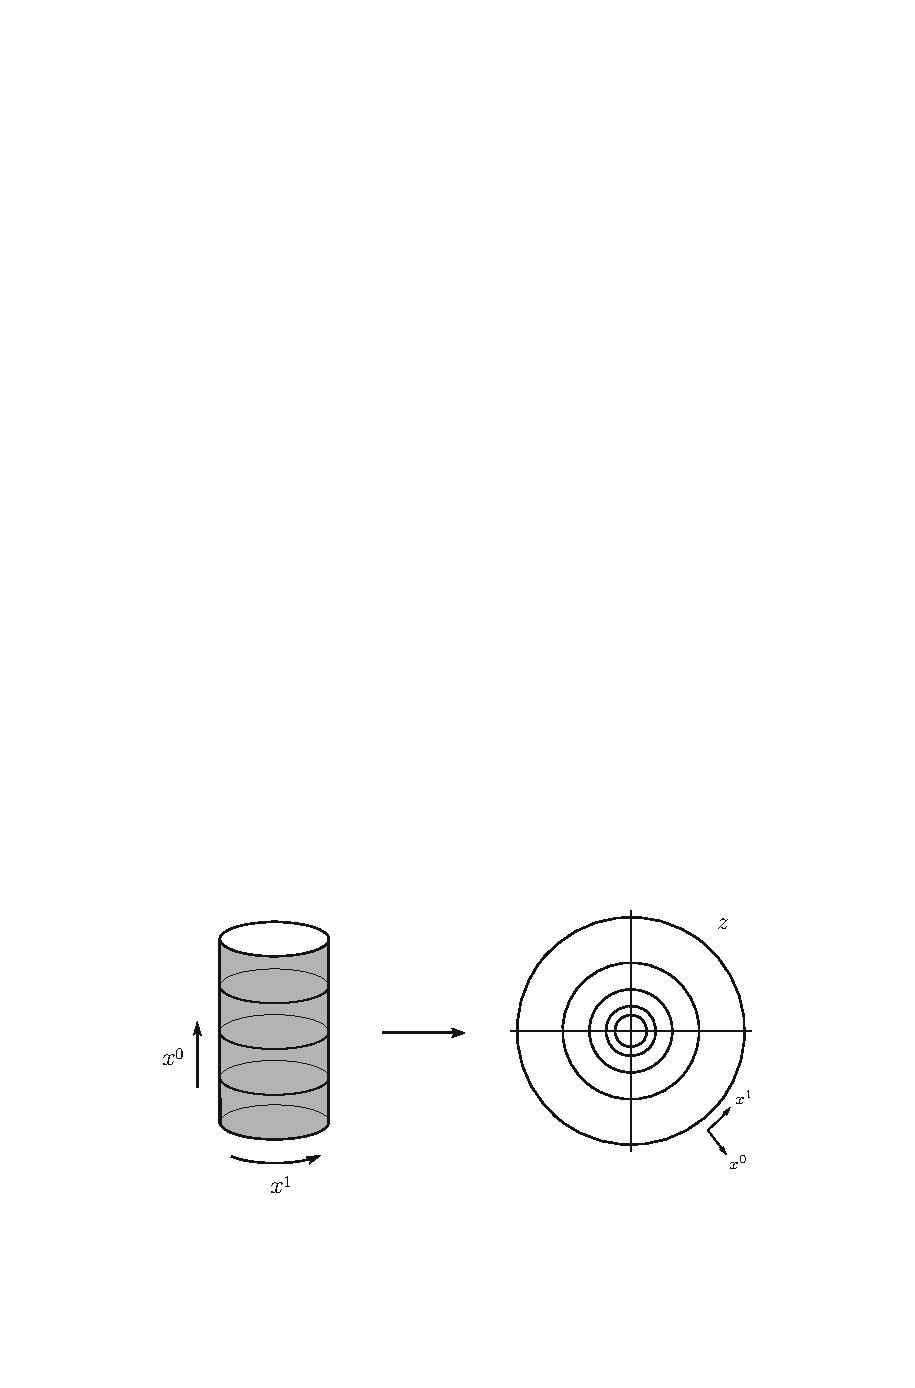
\includegraphics{figs/fig9.pdf}
	\caption{径向量子化}
\end{figure}
在这一变换下,时间方向变为了径向,空间方向变成了角向,而且把整个无穷远映射到了原点这一个点上。这下时间平移对应的哈密顿量$H$到复平面这边就变成了dilation算子$D$,而空间平移对应旋转$e^{i\theta}$:
\begin{equation}
		\boxed{H=L_0+\bar {L}_0,\quad P=i\left(=L_0-\bar {L}_0\right)}
\end{equation}
也正是因为时间方向变成了径向,时序积就应当变成“径向顺序积”,我们要去计算的就是径向顺序积的真空期望值,对于玻色子定义为:\sn{费米子把下面的情况改成负号就好}
\begin{equation}
	R\bigl(A(z)B(w)\bigr)\equiv\begin{cases}{}A(z)B(w)&\text{for }|z|>|w|,\\B(w)A(z)&\text{for }|w|>|z|.\end{cases}
\end{equation}

圆柱上的场我们用$\varphi(w,\bar w)$表示,复平面上的场用$\phi(z,\bar z)$表示,那么根据共形变换:
\begin{equation}
	\phi(z,\bar z)=z^{-h}{\bar {z}}^{-\bar h}\varphi(w,\bar w)
\end{equation}
在圆柱那边的CFT中我们知道$\varphi(w,\bar w)$可以做平面波展开为$e^{-ip^0x^0+ip^1x^1}$,由于我们考虑的是欧氏空间的场论,Wick转动后得到$e^{-p^0x^0+ip^1x^1}$,即$(e^{-w})^n(e^{-\bar w})^{\bar m}$的形式\sn{$n+m=p^0,n-m=p^1$}。而这恰恰就是洛朗展开的每一项!所以复平面上的CFT的模式展开为洛朗展开:
\begin{theorem}[Mode Expansion]
	\begin{equation}
		\boxed{\phi(z,\overline{z})=\sum_{n,\overline{m}\in\mathbb{Z}}z^{-n-h}\overline{z}^{-\overline{m}-\overline{h}}\phi_{n,\overline{m}}}
	\end{equation}
\end{theorem}
量子化场就是把$\phi_{n,\bar m}$量子化为算符,这些算符具有$(n,\bar m)$的权。

QFT微扰计算中一个非常重要的概念是渐近态,我们考虑的都是无穷远处的平面波入射经过复杂的相互作用后的平面波出射,微扰的角度看入射态就是在无穷远处的过去在真空附近施加一个扰动,也就是插入场算符,出射态也类似的这样做,这样就会自然出来时序积,然后LSZ约化这些的去计算振幅。同样的CFT这边也有这样的物理图景,只是现在无穷远处过去被映射到原点这一个点上了,所以渐近态应该定义为:
\begin{equation}
	ket{\phi}=\lim_{z,\overline{z}\to0}\phi(z,\overline{z})\ket{0}
\end{equation}
在原点处上式不奇异自然要求:\sn{这似乎告诉我们$n>-h,\bar m>-\bar h$对应的是CFT中的湮灭算符,后面讲到对易子会回到这里}
\begin{equation}\label{eq:30.6}
	\phi_{n,\overline{m}}\ket{0} =0\quad\text{for}\quad n>-h,\quad\overline{m}>-\overline{h}
\end{equation}
完整得到渐近态的公式:
\begin{equation}
	\boxed{|\phi\rangle=\lim\limits_{z,\overline{z}\to0}\phi(z,\overline{z})\left|0\right\rangle=\phi_{-h,-\overline{h}}\left|0\right\rangle}
\end{equation}
这里有个非常有趣的地方,本来一个算符里面有很多模,最后只剩下了一个,所以在CFT中,态和\textbf{局域}算符是唯一对应的!这就是态\mbox{-}算符对应。这和一般的QFT形成了鲜明的对比,那里一个场对应是不同“方向”平面波的组合,没有做到一一对应,但是CFT做到正是因为他把一个无穷大的空间部分在无穷远的过去全部紧化到了原点这一处,为了加深理解我们用路径积分的观点来看一下。

回忆量子力学中的传播子可以用路径积分表达为:
\begin{equation}
	G(x_f,x_i)=\int_{x(\tau_i)=x_i}^{x(\tau_f)=x_f}\mathcal{D}xe^{iS}
\end{equation}
那么演化后的末态波函数可以用初态波函数传播得到:
\begin{equation}
	\psi_{f}(x_{f},\tau_{f})=\int dx_{i}G(x_{f},x_{i})\psi_{i}(x_{i},\tau_{i})
\end{equation}
QFT这边“波函数”是一个泛函$\Psi[\phi(\sigma)]$,其模方表示在固定时间,空间中每个点$\sigma$上出现场构型$\phi(\sigma)$的概率,可以用路径积分得到末态:
\begin{equation}
	\Psi_f[\phi_f(\sigma),\tau_f]=\int\mathcal{D}\phi_i\int_{\phi(\tau_i)=\phi_i}^{\phi(\tau_f)=\phi_f}\mathcal{D}\phi e^{-S[\phi]}\Psi_i[\phi_i(\sigma),\tau_i]
\end{equation}
现在从柱面换到复平面CFT:
\begin{equation}
	\Psi_f[\phi_f(\sigma),r_f]=\int\mathcal{D}\phi_i\int_{\phi(r_i)=\phi_i}^{\phi(r_f)=\phi_f}\mathcal{D}\phi e^{-S[\phi]}\Psi_i[\phi_i(\sigma),r_i]
\end{equation}
不难发现初始态的作用是对$|z|=r_i$的积分进行加权,构造初始态需要在无穷远的过去,$r_i\to 0$,从而初始态只对原点处积分进行加权,等价于在原点处插入一个算子,即:
\begin{equation}
	\Psi[\phi_f;r]=\int^{\phi(r)=\phi_f}\mathcal{D}\phi e^{-S[\phi]}\mathcal{O}(z=0)
\end{equation}

\subsection{BPZ Conjugate}
为了构建关联函数,我们需要“左矢”,也就是厄米共轭来构造出射态从而有内积,这里谈的BPZ共轭是厄米共轭在Wick转动后的径向量子化欧氏空间CFT上的自然推广。不想扯过多物理上的考量,\cite{ito}从Wick转动后厄米共轭必须与时间反演一同定义BPZ共轭来解释了这一定义。
\begin{definition}[BPZ Conjugate]
	\begin{equation}
		\phi^\dagger(z,\overline{z})=\overline{z}^{-2h}z^{-2\overline{h}}\phi\left(\frac{1}{\overline{z}},\frac{1}{z}\right)
	\end{equation}
\end{definition}
另一方面直接从洛朗展开得到:
\begin{equation}
	\phi^{\dagger}(z,\overline{z})=\overline{z}^{-2h}z^{-2\overline{h}}\sum_{n,\overline{m}\in\mathbb{Z}}\overline{z}^{+n+h}z^{+\overline{m}+\overline{h}}\phi_{n,\overline{m}}=\sum_{n,\overline{m}\in\mathbb{Z}}\overline{z}^{+n-h}z^{+\overline{m}-\overline{h}}\phi_{n,\overline{m}}
\end{equation}
从而有:
\begin{equation}\label{BPZ}
	\boxed{
	\left(\phi_{n,\overline{m}}\right)^\dagger=\phi_{-n,-\overline{m}}
	}
\end{equation}
根据场的BPZ共轭定义,出射态应该定义为:
\begin{equation}
	\bra{\phi}=\lim\limits_{z,\overline{z}\to0}\bra{ 0  }              \phi^\dagger(z,\overline{z})=\lim\limits_{\overline{w},w\to\infty}w^{2h}\overline{w}^{2\overline{h}}\bra{0}\phi(w,\overline{w})=\bra{0}\phi_{h,\bar h}
\end{equation}
这里根据非奇异性要求了:
\begin{equation}\label{eq:30.17}
	\left<0\right|\phi_{n,\overline{m}}=0\quad\text{for}\quad n<h,\quad\overline{m}<\overline{h}
\end{equation}
当然,这里是根据定义严格来构造了一遍,实际计算疯狂使用\ref{BPZ}就好。
\section{Ward Identity and OPE}
\subsection{Infinitesimal Conformal Ward Identity}
前面$\S 4$已经看到共形对称性对应的守恒流可以使用$T_{\mu\nu}\epsilon^\nu$来构造,利用前面得到的最一般的Ward恒等式\ref{eq:19.11},对整个时空进行积分:
\begin{equation}
	\int dx^0dx^1\frac\partial{\partial x^{\mu}} \left\langle j_{a}^{\mu}(x)\Phi(x_{1})\cdots\Phi(x_{n})\right\rangle  =\sum_{i=1}^{n}\left<\Phi(x_{1})\delta_{\epsilon,\bar \epsilon}\cdots\Phi(x_{i})\cdots\Phi(x_{n})\right>
\end{equation}
$z=e^{x^0+ix^1}=x+iy$,进一步利用积分换元得到:\sn{别忘了雅可比行列式}
\begin{equation}
	\begin{aligned}
		\int dx^0dx^1&\partial_\mu\left\langle j_{a}^{\mu}(x)\Phi(x_{1})\cdots\Phi(x_{n})\right\rangle\\
		&=4\int dzd\bar z\left[\bar\partial(T_{\bar z\bar z}\epsilon)+\partial(T_{zz}\bar\epsilon)\right]\\
		&=2\int dxdy\left[\bar\partial(T_{\bar z\bar z}\epsilon)+\partial(T_{zz}\bar\epsilon)\right]
	\end{aligned}
\end{equation}
上面取了约定$\epsilon^z\equiv\epsilon(z),\partial_z\equiv\partial$,反全纯部分类似。现在考虑二元积分的格林公式:
\begin{equation}
	\begin{aligned}\oint_{\partial\Omega}P(x,y)dx+Q(x,y)dy=\int_\Omega dxdy\left(\frac{\partial Q}{\partial x}-\frac{\partial P}{\partial y}\right)\end{aligned}
\end{equation}
利用复变量$z=x+iy$可得下面的形式:\sn{就像是Wick转动一样,我们总假设这样随意复化是可行的}
\begin{equation}
	\begin{aligned}\oint_{\partial_\Omega}frac{1}{2}(P-iQ)dz+\frac{1}{2}(P+iQ)d\bar{z}=\int_\Omega dxdy(\partial(Q-iP)+\bar{\partial}(Q+iP))\end{aligned}
\end{equation}
上式中所有的围道积分都假设方向相对于$z$而言是逆时针,那么在$\bar z$平面上也就是逆时针,不过为了方便,而且CFT中我们也只考虑全纯部分,反全纯部分只要做个Conjugate就好了,后文中$\oint d\bar z$,表示围道方向相对于$\bar z$逆时针。
\begin{equation}
	\int_\Omega dxdy\left(\partial \bar f+\bar\partial f\right)=\frac{1}{2i}\oint_{\partial\omega}fdz+\bar f d\bar z
\end{equation}
再取:
\begin{equation}
	T(z)\equiv-2\pi iT_{zz},\bar T(\bar z)\equiv-2\pi iT_{\bar z\bar z}
\end{equation}
不过这个归一化因子并不重要,只是为了让OPE有一般的convention,后面比如自由玻色子这些具体模型我们都是先将归一化因子待定,再根据OPE的形式来确定它,只需要记住二维共形场论中$T_{zz}$始终全纯,$T_{\bar z\bar z}$始终反全纯就好了。归一化能动张量后,得到初级场的Ward恒等式:
\begin{equation}\label{ward}
	\boxed{
	\sum_{i=1}^{n}\left<\Phi(x_{1})\cdots\delta_{\epsilon,\bar \epsilon}\Phi(x_{i})\cdots\Phi(x_{n})\right>=\frac{1}{2\pi i}\oint\left\langle\left(T(z)\epsilon(z)dz+\bar T(\bar z)\bar \epsilon(\bar z)d\bar z\right)\Phi(x_{1})\cdots\Phi(x_{i})\cdots\Phi(x_{n})\right\rangle
	}
\end{equation}
这里积分围道包围所有$w_i$。根据上式我们可以定义\textbf{Conformal charge}:
\begin{equation}
	Q\equiv\frac{1}{2\pi i}\oint_{\mathcal{C}}\Bigl(dzT(z)\epsilon(z)+d\overline{z}\overline{T}(\overline{z})\overline{\epsilon}(\overline{z})\Bigr)
\end{equation}
这样便有:
\begin{equation}\label{eq:31.9}
	-\delta_{\epsilon,\bar\epsilon}\Phi=\left[Q,\Phi\right]
\end{equation}
\subsection{Operator Product Expansion}
但是\ref{eq:31.9}表面上有个非常大的漏洞,那就是因为全纯,直接导致围道积分始终为0。解决这一问题是注意到Q是一个算符,需要作用到其它场上面,而两个算符靠的非常近时真空涨落发散\sn{类似于$a_p,a_p^\dagger\sim\delta(0)$},上式积分中出现极点。也正是极点的存在导致我们定义局域算符之间的对易子的时候需要做正规化:
\begin{equation}
	[A(z,\bar{z}),B(w,\bar{w})]=\lim_{\begin{smallmatrix}|z|\rightarrow|w|\\|z|>|w|\end{smallmatrix}}A(z,\bar{z})B(w,\bar{w})-\lim_{\begin{smallmatrix}|z|\rightarrow|w|\\|w|>|z|\end{smallmatrix}}B(w,\bar{w})A(z,\bar{z})
\end{equation}
这直接导致对易子的计算可以等价于对径向顺序积的计算:\sn{后文中$\mathcal{C}(w)$表示只绕$w$的逆时针围道}
\begin{equation}
	\boxed{\begin{gathered}
			\oint dz\bigl[A(z),B(w)\bigr] =\oint_{|z|>|w|}dzA(z)B(w)-\oint_{|z|<|w|}dzB(w)A(z) \\
			=\oint_{\mathcal{C}(w)}dzR\Big(A(z)B(w)\Big), 
	\end{gathered}}
\end{equation}
现在利用只含一个初级场的无穷小变换Ward恒等式,或者说\ref{eq:31.9},注意到\ref{ict},以及:\sn{回忆$n$阶极点留数公式:\[\begin{aligned}
		\operatorname{Res}&[f(z),a]\\=&\lim\limits_{z\to a}\frac{1}{(n-1)!}\frac{d^{n-1}}{dz^{n-1}}\left[(z-a)^nf(z)\right]
	\end{aligned}\]}
\begin{equation}\label{eq:31.12}
	\begin{gathered}
		h\left(\partial_{w}\epsilon(w)\right)\phi(w,\overline{w}) =\frac{1}{2\pi i}\oint_{\mathcal{C}(w)}dzh\frac{\epsilon(z)}{(z-w)^{2}}\phi(w,\overline{w}), \\
		\epsilon(w)\left(\partial_{w}\phi(w,\overline{w})\right) =\frac1{2\pi i}\oint_{\mathcal{C}(w)}dz\frac{\epsilon(z)}{z-w}\partial_{w}\phi(w,\overline{w}).
	\end{gathered}
\end{equation}
得到全纯部分:
\begin{equation}
	R\left(T(z)\phi(w,\overline{w})\right)=\frac{h}{(z-w)^2}\phi(w,\overline{w})+\frac{1}{z-w}\partial_w\phi(w,\overline{w})+\ldots 
\end{equation}
\textbf{后面的省略号表示非奇异的项},大多数情况下我们要用的是OPE的奇异部分,因为它完全包含了和对易子一样的信息。像这样的把算符展开成其它算符和的形式称为\textbf{OPE}。在一般的QFT中我们计算时序积需要先写下路径积分,然后进行微扰展开算费曼图,但是CFT中我们只需要去考虑OPE就好了,对称性为我们简化了许多。后面写OPE会省略$R(\cdot)$,利用算符和能动张量之间的OPE我们还能给出一个初级场的等价定义:
\begin{theorem}
	一个场是共形权为$(h,\bar h)$的初级场\textbf{当且仅当}它满足:
	\begin{equation}
		\boxed{\begin{gathered}
				T(z)\phi(w,\overline{w}) =\frac{h}{(z-w)^{2}}\phi(w,\overline{w})+\frac{1}{z-w}\partial_{w}\phi(w,\overline{w})+\ldots  \\
				\overline{T}(\overline{z})\phi(w,\overline{w}) =\frac{\overline{h}}{(\overline{z}-\overline{w})^{2}}\phi(w,\overline{w})+\frac{1}{\overline{z}-\overline{w}}\partial_{\overline{w}}\phi(w,\overline{w})+\ldots  
		\end{gathered}}
	\end{equation}
\end{theorem}
再次强调,之后写下的所有的OPE都应当认为是在在时序关联函数中插入算符时成立的关系!而且因为是时序积之中的关系:
\begin{equation}
	\langle\mathcal{O}_i(z,\bar{z})\mathcal{O}_j(w,\bar{w})\ldots\rangle=\sum_kC_{ij}^k(z-w,\bar{z}-\bar{w})\langle\mathcal{O}_k(w,\bar{w})\ldots\rangle 
\end{equation}
所以OPE结合律和交换律都自动满足。上式中$\ldots$表示其它任意算符的插入,当然既然是级数总有一个收敛半径,何时OPE的插入是有效的是我们需要关心的,从前面对OPE的推导可以看出我们要求积分围道中只有$w$这一个奇点,所以OPE是精确的当且仅当其它算符的插入点$\{w_i\}$满足$|w-w_i|>|z-w|$。

现在再回到Ward恒等式\ref{ward},但是现在考虑有多个$\Phi$的插入,从前面对OPE的分析得知围道内的极点是$\{w_i\}$,然后利用柯西定理将等式右边的积分换成对绕每个极点的围道积分求和得到:
\begin{equation}
	\begin{aligned}0=\oint\frac{dz}{2\pi i}\epsilon(z)&\Bigg[\Big\langle T(z)\phi_1(w_1,\overline{w}_1)\ldots\phi_N(w_N,\overline{w}_N)\Big\rangle\\
		&-\sum_{i=1}^N\left(\frac{h_i}{(z-w_i)^2}+\frac{1}{z-w_i}\partial_{w_i}\right)\Big\langle\phi_1(w_1,\overline{w}_1)\ldots\phi_N(w_N,\overline{w}_N)\Big\rangle\Bigg]\end{aligned}
\end{equation}
等式左边再次利用\ref{eq:31.12},得到所谓共形Ward恒等式(仅适用于初级场):\sn{注意这并不是代入$T,Phi$之间OPE得到的,因为前面说过OPE收敛半径等于与OPE处最近的其他算符插入处的距离。而我们下面要导出的等式与算符插入点完全无关,推导过程中看到我们将围道变形为单独绕每个$\{w_i\}$的围道来使得OPE的插入是精确的。}
\begin{equation}
	\boxed{\begin{aligned}\big\langle T\left(z\right)&\phi_{1}(w_{1},\overline{w}_{1})\ldots\phi_{N}(w_{N},\overline{w}_{N})\big\rangle\\&=\sum_{i=1}^{N}\left(\frac{h_{i}}{(z-w_{i})^{2}}+\frac{1}{z-w_{i}}\partial_{w_{i}}\right)\Big\langle\phi_{1}(w_{1},\overline{w}_{1})\ldots\phi_{N}(w_{N},\overline{w}_{N})\Big\rangle\end{aligned}}
\end{equation}
\subsection{n-point correlators (n<4)}
利用共形对称性实际上可以完全确定四点以下关联函数的形式。先来考虑准初级chiral场的关联函数,前面考虑的都是无穷小变换的Ward恒等式,但实际上在这里我们要使用的只是有限global共形变换的Ward恒等式,一般形式如下:
\begin{equation}\label{global ward}
	\boxed{
	\langle\phi_1'(x_1')\cdots\phi_N'(x_N')\rangle=\langle\phi_1(x_1')\cdots\phi_N(x_N')\rangle
	}
\end{equation}
上式等价于:
\begin{equation}
	\left\langle\phi_{1}\left(z_{1},\bar{z}_{1}\right)\cdots\phi_{n}\left(z_{n},\bar{z}_{n}\right)\right\rangle=\prod_{i=1}^{n}\left(\frac{\partial z'}{\partial z}\right)^{h_{i}}\left(\frac{\partial\bar{z}'}{\partial\bar{z}}\right)^{\bar{h}_{i}}\Bigg|_{z=z_{i},\bar{z}=\bar{z}_{i}}\left\langle\phi_{1}\left(z'_{1},\bar{z}'_{1}\right)\cdots\phi_{n}\left(z'_{n},\bar{z}'_{n}\right)\right\rangle 
\end{equation}
可以通过考察路径积分轻易得到。利用这一等式就可以得到一点关联函数必定是trivial的,这也可以根据前面的态算符对应要求的\ref{eq:30.6}\ref{eq:30.17}得到。
\begin{theorem}[2-pt]
	\begin{equation}\label{31.19}
		\left\langle\phi_i(z)\phi_j(w)\right\rangle=\frac{d_{ij}\delta_{h_i,h_j}}{(z-w)^{2h_i}}
	\end{equation}
\end{theorem}
\begin{theorem}[3-pt]
	\begin{equation}\label{31.20}
		\left\langle\phi_1(z_1)\phi_2(z_2)\phi_3(z_3)\right\rangle=\frac{C_{123}}{z_{12}^{h_1+h_2-h_3}z_{23}^{h_2+h_3-h_1}z_{13}^{h_1+h_3-h_2}}
	\end{equation}
	其中$z_{ij}\equiv z_i-z_j$
\end{theorem}
另外根据关联函数的单值性,还进一步要求\sn{后面考虑Virasoro代数表示的时候我们会先暂时忘掉这个要求。}\textbf{Chiral场的共形权只能是整数或者半整数}。把反全纯部分也加进来考虑得到:
\begin{itemize}
	\item 2-pt:
	\begin{equation}
		\left\langle\phi_1(z_1,\overline{z}_1)\phi_2(z_2,\overline{z}_2)\right\rangle=\frac{d_{12}}{z_{12}^{h_1+h_2}\overline{z}_{12}^{\overline{h}_1+\overline{h}_2}}\delta_{h_1,h_2}\delta_{\overline{h}_1,\overline{h}_2}
	\end{equation}
	\item 3-pt:
	\begin{equation}
		\begin{aligned}\big\langle\phi_1(z_1,\overline{z}_1)&\phi_2(z_2,\overline{z}_2)\phi_3(z_3,\overline{z}_3)\big\rangle\\&=\frac{C_{123}}{z_{12}^{h_1+h_2-h_3}z_{23}^{h_2+h_3-h_1}z_{13}^{h_1+h_3-h_2}\overline{z}_{12}^{\vec{h}_1+\vec{h}_2-\vec{h}_3}\overline{z}_{23}^{\vec{h}_2+\vec{h}_3-\vec{h}_1}\overline{z}_{13}^{\vec{h}_1+\vec{h}_3-\vec{h}_2} }\end{aligned}
	\end{equation}
\end{itemize}

关于这些公式的详细推导\cite{ito}上面都有,这里主要考虑用无穷小Ward恒等式的方法,但是我们考虑的毕竟是准初级场,所以只需要考虑$\epsilon(z)=\epsilon_{-1}+\epsilon_0z+\epsilon_1z^2$。将\ref{global ward}在无穷小变换下展开得到全纯部分:
\begin{equation}
	\displaystyle\sum_{i=1}^{n}\left(h_{i}\partial_{i}\epsilon\left(z_{i}\right)+\epsilon\left(z_{i}\right)\partial_{i}\right)\left<\phi_{1}\left(z_{1}\right)\cdots\phi_{n}\left(z_{n}\right)\right>=0+\mathcal{O}(\epsilon^2)
\end{equation}
这是一个微分方程,对于$\epsilon(z)=\epsilon_{-1}+\epsilon_0z+\epsilon_1z^2$恒成立,所以我们可以通过求解这个微分方程来确定关联函数的形式,不难验证\ref{31.19}和\ref{31.20}就有这一特征。这种将关联函数计算转化为微分方程的求解的方法后面我们还会碰到。

但是四点及以上函数就不能确定到只差一个待定系数了,不过我们仍旧可以利用所谓\textbf{交叉对称性}(Crossing Symmetry)走的很远。

\subsection{General Form of the OPE}

\section{NOPs and Conformal family}
\subsection{Normal Ordered Products}
\subsection{Verma module}
\subsection{Descendant states}
\section{Crossing Symmetry}